\section{Introduction}
In this chapter, we will present the different software components that were combined together to build our system. Problems with engineering and platform complexity will be highlighted, along with the process for solving them. The Android operating system brings many challenges with regards to development; however the goal is to explain those which are interesting when developing solutions relating to NFC. A basic knowledge of the Android platform will prove useful to fully understand this chapter.
\section{Primary Technology}
As explained earlier (blah blah reference), Stamped is to be developed on a popular mobile platform that supports the NFC standard, in this case Android. At this moment in time, developing a functional prototype for this system cannot be possible on another platform due to hardware and API limitations regarding NFC and Host Card Emulation. Expanding the solution to external platforms in the future will be difficult as it requires a rewrite with platform-specific code.
\subsection{Software}
Google provides a plethora of development tools in order to develop applications, one such tool is the development environment \emph{Android Studio}. This kit provides an Integrated Development Environment (IDE) in order to design, configure and program the system. Android programs are coded using \texttt{JAVA} -- therefore requiring an object oriented methodology. 

Different Android devices run different versions of the operating system. Corresponding to each operating system version, there exists an accompanying Application Program Interface (API) that introduces new features to the ecosystem. We want our application to have the highest compatibility, but still contain the required features in order to satisfy the requirements. \emph{Android 4.4 KitKat} is selected as this is when Host Card Emulation was initially introduced into the platform; however, this means that approximately 45\%~\cite{Androidusagestats} of Android users have an appropriate version of operating system to run Stamped.

\subsection{Hardware}
Complementing the above choice of software, we require accommodating Android devices for development. Two devices were selected, a smartphone and a tablet. The tablet will be used to implement the Stamped Manager application as businesses will ideally mount Tablets onto a table next to employees to use. On the other hand, the phone will be used for the Stamped application as this is the common device customers will be using the system with. Both devices run the latest \emph{Android 5.0 Lollipop} operating system - therefore supporting Host Card Emulation. 

\section{Other Notable Resources}
\subsection{Webserver with Database}
To facilitate the backend of the system, we introduced a webserver/database backend in the design. A private webserver was purchased in order to facilitate the interactions with the database. The design database schema (Ref. SCHEMA) was imported into \emph{PHPMyAdmin} and PHP files were developed to interface between the Applications and Webserver (The rationale for this can be found in (Sec. \ref{sec:databasecommunication}))

\subsection{Android Debug Bridge (ADB)}
Google provides a useful software for application testing called The Android Debug Bridge. This software interfaces with connected devices, providing the following features.
\begin{itemize}
 \item The ability to see the console of the Android device in real-time whilst running the software
  \item The ability to control in-ward and out-bound network connections
   \item Error identification and debug output
\end{itemize} 

ADB persists whenever there is a connection between Android Studio and a device, outputting feedback on its current state.

\section{Implementation Complications}
In this section a discussion follows the key implementation complexities whilst developing the system. Care was taken to abstract the problems of developing on the Android platform away from the issues.
\subsection{Host Card Emulation}
We earlier defined a need for an interaction architecture, identifying the Stamped application to interact using HCE as a smartcard. In order to do achieve this, a service will need to be created 

\newpage{}

\subsubsection{Creating The Service}
In order to provide functionality outside of an application, a `service' must be implemented. A service is simply a component of an application which constantly runs in the background -- Host Card Emulation is one such example of a component. In this case, the HCE service passively runs in the phone working memory, waiting to be triggered by an NFC Reader before sending a message. The purpose of having HCE in this form allows users to tap a reader to collect stamps \textbf{regardless of whether the application is open on the device or not}.

Android services must be carefully developed, as reckless design will lead to unwanted battery drain on the device. Fortunately Google provides a template class called \emph{HostApduService} for HCE, ensuring that the service is optimised for power consumption. 

\subsubsection{Distinguishing Actions}
A standard smartcard cannot tell what exactly is being read from it or when, a similar problem presents itself in the Host Card Service. The HCE service cannot atomically discriminate what message it needs to send, it can only react to an \texttt{onRead} event. To remediate this, we had to temporarily break the object oriented principle of encapsulation by introducing a shared global variable \texttt{NFCMessageType}. The message will allow the Manager application to discriminate what type of action we are broadcasting as a smartcard. Two such messages are adopted:
\begin{enumerate}
 \item Stamp mode - Broadcasts the user account id
  \item Reward mode - Broadcasts the user account id, the scheme id and the number of stamps to deduct in order to claim that reward
\end{enumerate}
Passively the device is on `Stamp' mode; however once a user selects a reward, they are presented with a popup (Fig. \ref{fig:extrinsicmotivation}) to tap the reader in order to claim their reward. During this time, the HCE service will be in `Reward' mode. As the popup is dismissed (from tapping the reader or having the user press cancel), we return back to Stamp mode. This technique underlies the systems ability to Understand Actions (Sec. \ref{sec:understanding}).

\begin{figure}[H]
 \centering
  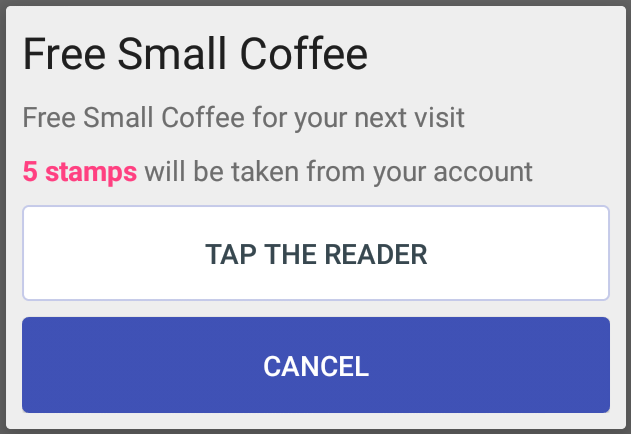
\includegraphics[width=0.40\textwidth]{img/claimreward.png}
     \caption{The popup presented to the user when they are about to claim a reward}
     \label{fig:claimreward}
\end{figure}

\subsubsection{Reacting to OnRead}
The \texttt{onRead} function is usually strictly used to send a message to a reader. However, the event affords many opportunities for us to implement user feedback mentioned in the design chapter. For instance, we announce to the user whenever they have tapped their device using audio feedback and a notification (Fig. \ref{fig:notification}). This novel solution binds the interaction feedback to the service; therefore these functions can run in the background.

\begin{figure}[H]
 \centering
  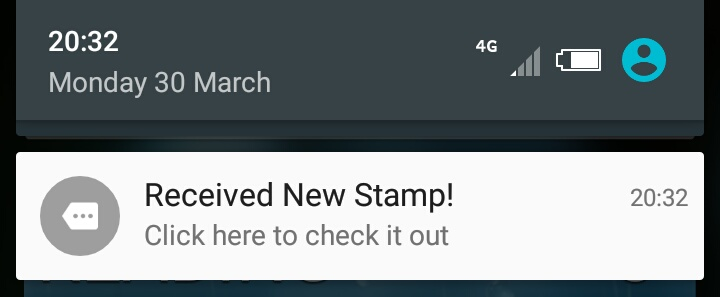
\includegraphics[width=0.40\textwidth]{img/notification.jpg}
     \caption{A Notification providing feedback to the user upon receiving a stamp}
     \label{fig:notification}
\end{figure}

\subsection{NFC Communications}
Several presentation methods need to be put in place to facilitate NFC communication for our system. The messages being sent are simply hexadecimal plaintext; therefore there needs to be a way to send them in the correct format and carry some meaning to them. Here we demonstrate the principles to enable the Stamped Manager to understand messages.

\subsubsection{Understanding Actions}
\label{sec:understanding}
The Stamped Manager must be able to distinguish the types of messages it receives. There are two kinds that it may encounter: A stamp request and a reward claim. We earlier explained two modes on the host card that send differing amounts of information. Likewise, the Manager was setup in order to analyse message content. If only the accountID was received, we know that Stamped Manager needs to provide a stamp, however when is presented with more information, the system recognises that a customer is claiming a reward and deducts the amount of stamps from their account.

\subsubsection{Avoiding the `Beam'}
Android Beam is a feature of the Android platform to allow peer-peer data exchange over NFC~\cite{androidBeam}. Though it may have its uses (i.e Sending contacts, pictures), it can cause many problems for our system. Primarily, when two devices `tap', the operating system may mistake it for a `Beam' instead of a smartcard. This feature can be seen in (Fig. \ref{fig:androidBeam}); however we draw attention to the message which says `Touch to beam'. When this message appears, any input to the device other than that specific action is blocked. This will naturally clash with the Stamped Manager, which is expecting a host card message instead of a `Beam'

To solve this problem, we had to implement tight controls over how the Manager enables and disables its NFC chip, only enabling the chip whilst the reader is listening for a message from a host card.

\begin{figure}[H]
 \centering
  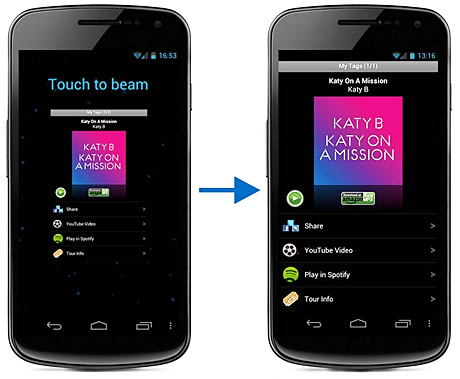
\includegraphics[width=0.40\textwidth]{img/androidBeam.jpg}
     \caption{A demonstration of Android beam}
     \label{fig:androidBeam}
\end{figure}

\subsubsection{ApplicationID Filtering}
An Android device can emulate many smartcards simultaneously; however this is an issue for a NFC Reader as it will not be able to distinguish between the smartcards. We solve this issue through ApplicationID (AID) Filtering. Whenever a host card is setup, an ApplicationID must be assigned to it in the form of a hexadecimal string. An NFC Reader application can apply an AID filter with a matching hexadecimal string (Fig. \ref{fig:aidfilter}) in order to identify and accept only the intended smartcard.

\begin{figure}[H]
 \centering
  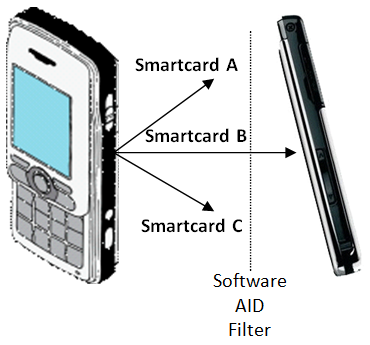
\includegraphics[width=0.40\textwidth]{img/aidfilter.png}
     \caption{A schematic demonstrating software AID Filtering}
     \label{fig:aidfilter}
\end{figure}

\subsection{Database Communication}
\label{sec:databasecommunication}
A large part of the system interactions involve reporting back to the central database in order to sync `stampbooks' along with user profiles. We deduced during the design stage that only the Stamped Manager will have access to modify entries in the database, whereas the user Stamped application will only be able to read from it -- A discussion follows on the implementation of database communication for our system.
\subsubsection{PHP Interface}
Interfacing directly with SQL is highly difficult and insecure in the Android platform. To solve this a new interface had to be made using PHP. In this architecture, applications send \texttt{GET} and \texttt{PUT} requests to the server, identifying actions by using `tags'. PHP in turn works as an intermediary, sending input to the database and providing output back to the Android application. Unfortunately this means that functions have to be written essentially twice, as they need to be written in JAVA to call a PHP, along with being written PHP to handle the input/output.
\subsubsection{Database Requests}
%UI THREAD NONONO
Requests to the database take time, and therefore must be threaded properly on mobile platforms. Android is very strict with regards requests what is allowed to run on the UI Thread. Requests that are recognised to be time consuming (i.e. Database requests) must be setup to run on a separate thread of execution. The adverse side effect of this requirement introduced the problem of race conditions in our UI.
\subsubsection{Dealing With Race Conditions in the UI}
Consider the following example -- A user is syncing their `stampbook' to see how many stamps they have for each of their loyalty schemes. The request runs in a background thread; however it does not update the new stamp values as they have already been drawn on screen. We fix this by constantly updating the views every few seconds. This solution was not ideal, nonetheless it did remediate our race conditions.

\newpage

\subsection{Internal Database Management}
Storing information on Android can be non-intuitive. Basic credentials can be cached through plain text files; but in order to store the complex inter-relating data of our system. An internal database needs to be deployed to serve as local storage. Here we outline the novel challenges when working with both an internal and online database.
\subsubsection{The Internal Database}
Information gathered from querying the online database has to be stored somewhere, as a result, a \texttt{SQLite} database is setup with an identical schema. The idea is to have a clone of the parts relevant to the user (i.e. Account details, loyalty schemes, available rewards) of the online database stored locally. This vastly reduces the number of database calls that need to be made, as well as solving our information storage problem. On the other hand, it adds an extra layer of complexity as some SQL queries will still need to be run on the internal database \textbf{as well as} the online database. 
%Syncing between Internal and Online backup
\section{Delivery of Requirements}
Here we will compare how well the implemented system delivered on our earlier requirements.

\subsection{Overview}
Here we show a high-level overview of how many MoSoCoW requirements were completed. 
\begin{itemize}
	\item Must Have -- 7/7
	\item Should Have -- 3/6
	\item Could Have -- 5/7
	\item Wont Have -- 0/2
\end{itemize}

\subsection{Requirement Fulfillment}
\begin{description}[leftmargin=!,labelwidth=\widthof{\bfseries Medium}]
    \item[M1] \textbf{Sign-In \& Registration} \newline
        \textit{Users are able to sign-in to the system with their accounts}
        
    \item[M2] \textbf{Fast Stamping} \newline
        \textit{Stamping in the adopted design is pervassive; therefore no buttons on the user interface is needed. Any tap on a listening reader will provide a stamp.}
    
    \item[M3] \textbf{NFC Transmission} \newline
        \textit{Host Card Emulation is used to send messages over NFC.}
        
    \item[M4] \textbf{Online Syncing} \newline
        \textit{The system actively syncs the status of user `stampbooks' with the online database.}
        
    \item[M5] \textbf{Sync on Interaction} \newline
        \textit{The \texttt{onRead} event triggers a sync with the database whenever an interaction between two devices take place}
        
    \item[M6] \textbf{Syncing Time} \newline
        \textit{A fast backend and grouped data in the \texttt{JSON} format affords fast syncing.}
        
    \item[M7] \textbf{Feedback on Interaction}
        \textit{The system provides an audible sound and a notification whenever an interaction occurs.}

    \item[S1] \textbf{Consistency} \newline
        \textit{The system user interface was implemented using Google's Material Design.}
        
    \item[S2] \textbf{Rewards Browsing} \newline
        \textit{There is a dedicated rewards tab to allow users to browse all available rewards for a loyalty scheme.}

    \item[S3] \textbf{Badges} \newline
        \textit{Users are able to collect standard badges which earn a user `title'.}
     	
    \item[C1] \textbf{Passive Card Emulation} \newline
        \textit{The system does use passive host card emulation.}

    \item[C2] \textbf{Branding} \newline
        \textit{Some customisation options are available to schemes; however no frontend for them was implemented}

    \item[C3] \textbf{Internet-Free Stamping} \newline
        \textit{Only Stamped Manager requires an internet connection in order to provide a stamp. Customers can sync their stampbook whenever they have an internet connection to update their local stampbook.}
        
    \item[C4] \textbf{Multiple Device Support} \newline
        \textit{Having an online database affords the use of using your account on multiple devices - moreover they will be synced with eachother}
        
    \item[C5] \textbf{User Personalisation} \newline
        \textit{Our system allows the personalisation of profile pictures and user-earned `titles'.}
\end{description}

\newpage

\section{Design Conformance}
By following the criteria laid out in the design chapter, we managed to successfully produce two android applications which allow users to do the following:

\begin{enumerate}
	\item Collect stamps for corporate loyalty schemes
	\item Track progress of all loyalty schemes in real-time
	\item Expend stamps in order to claim rewards
	\item Collect badges to improve customer engagement
\end{enumerate} 

\section{Conclusion}
Throughout this chapter, we have concentrated on implementing a system in order to meet our requirements and design specifications. In the next chapter, we will introduce and perform a user field study to assess the system in a natural environment.